\documentclass[12pt, a4paper]{article}

\title{\textsc{Computer Architecture} Homework 4}
\author{110062219}
\date{\today}

\usepackage{amsmath}
\usepackage{amssymb}
\usepackage{caption}
\usepackage{subcaption}
\usepackage{tikz}
\usepackage{pgfplots}
\usepackage{listings}
\usepackage{float}
\usepackage{tabularx}
\usepackage{makecell}
\usepackage{hyperref}
%\usepackage{geometry}[margin=2cm]

\lstset{
  breaklines=true,
  basicstyle=\ttfamily,
}

\definecolor{nthu}{HTML}{7F1084}

% \renewcommand{\ttdefault}{pcr}

\begin{document}

\maketitle

\tableofcontents

\section{Assembly Coding}

\subsection{Evidence of Correctness}

\begin{figure}[H]
\centering
\includegraphics[width=\linewidth]{tc1}
\caption{Testcase 1}
\label{fig:tc1}
\end{figure}

\begin{figure}[H]
\centering
\includegraphics[width=\linewidth]{tc2}
\caption{Testcase 2}
\label{fig:tc2}
\end{figure}

\pagebreak[4]

In addition, I generated a testcase of length 25 and also pass it.

\begin{figure}[htbp]
\centering
\includegraphics[width=\linewidth]{tc0}
\caption{Testcase 0}
\label{fig:tc0}
\end{figure}

In fact, I came up with the assembly codes from C codes degree by degree. So I submitted my vary low-level, assembly-like, i.e., to name variables after registers and use \texttt{goto} and labels instead of loops, \href{https://atcoder.jp/contests/dp/submissions/41496401}{C codes} to AtCoder and got accepted to ensure the correctness.

\subsection{Flowchart}

First, I store the address of $arr$ in \texttt{a0} and $n$ in \texttt{a1}. By means of technique similar to \textbf{rolling array}, we needn't maintain the whole $dp$. Instead, we only need keep track of the 3 recent elements of $dp$, which are stored in \texttt{s0}, \texttt{s1} and \texttt{s2}, respectively. Likewise, I only record the 3 recent elements of $arr$ in \texttt{s3}, \texttt{s4} and \texttt{s5}, respectively, and advance \texttt{a0}, recede \texttt{a1} each time in loops.

The most notable part of my codes is that, as a competitive programmer, I tend to calculate the minimum and abstract values by fancy and elegant \textbf{bitwise operations} rather than \textbf{branches}. Due to 2's complement, we have $$\min\{l,r\}=r\oplus((l\oplus r)\land-(l<r))$$ and $$|x|=(x\oplus(x\gg(\text{sizeof}(x)\times\text{BYTE\_BITS}-1)))-(x\gg(\text{sizeof}(x)\times\text{BYTE\_BITS}-1))$$.

\begin{figure}[htbp]
\centering
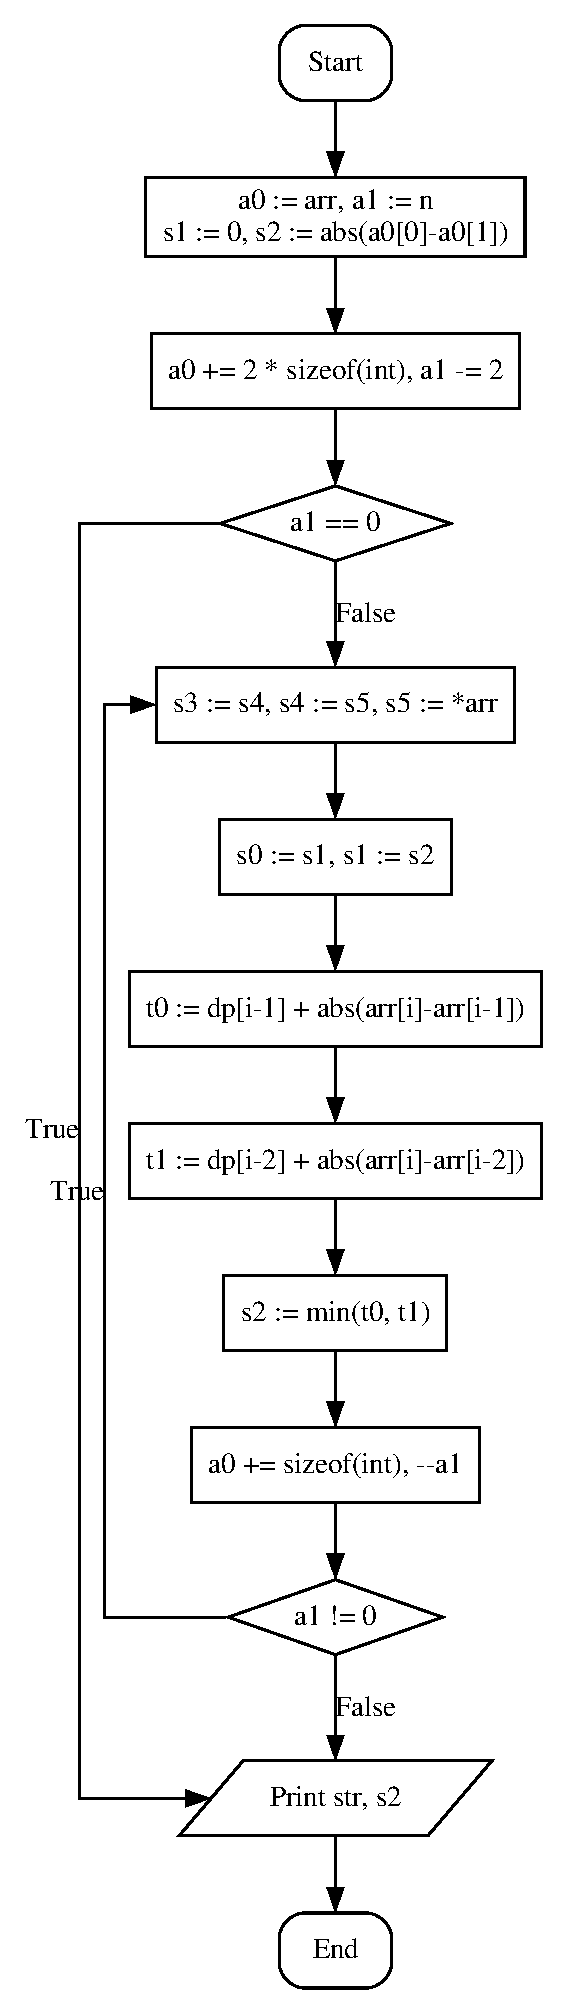
\includegraphics[width=.4\linewidth]{flowchart}
\caption{Flowchart}
\label{fig:fc}
\end{figure}

\section{Hazards in Codes}

\subsection{R-type RAW (EX)}

The \texttt{srai} instruction at line 38 reads the register \texttt{s2} as its first operand, which is written by the \texttt{sub} instruction at line 36. As a consequence, an EX hazard would occur.

In this case, the forwarding unit would set the signal \texttt{alu\_reg1\_forwarding\_ctrl} to be \texttt{MemStage}.

\begin{figure}[htbp]
\centering
\includegraphics[width=\linewidth]{1}
\caption{Type 1}
\label{fig:1}
\end{figure}

\pagebreak[4]

\subsection{R-type RAW (MEM)}

The \texttt{xor} instruction at line 39 reads the register \texttt{s2} as its first operand, which is written by the \texttt{sub} instruction at line 36. Therefore, a MEM hazard would occur.

In this case, the forwarding unit would set the signal \texttt{alu\_reg1\_forwarding\_ctrl} to be \texttt{WbStage}.

\begin{figure}[htbp]
\centering
\includegraphics[width=\linewidth]{2}
\caption{Type 2}
\label{fig:2}
\end{figure}

\pagebreak[4]

\subsection{Load RAW Immediately}

The \texttt{sub} instruction at line 36 reads the register \texttt{s5} as its second operand, which is written by the \texttt{lw} instruction at line 35. Accordingly, a load-use hazard would occur.

In this case, the hazard unit have to reset the signal \texttt{hazardFEEnable} to stall the pipeline, inserting a \texttt{nop} bubble between the two instructions. And then, in the next cycle, the forwarding unit would set the signal \texttt{alu\_reg2\_forwarding\_ctrl} to be \texttt{WbStage}.

\begin{figure}[htbp]
\begin{subfigure}{\linewidth}
\centering
\includegraphics[width=.88\linewidth]{3a}
\caption{}
\label{fig:3a}
\end{subfigure}
\begin{subfigure}{\linewidth}
\centering
\includegraphics[width=.88\linewidth]{3b}
\caption{}
\label{fig:3b}
\end{subfigure}
\caption{Type 3}
\label{fig:3}
\end{figure}

\subsection{Load RAW Between One Instruction}

The \texttt{sub} instruction at line 57 reads the register \texttt{s5} as its first operand, which is written by the \texttt{lw} instruction at line 52. (There are 2 blank lines and a comment line in between.) Whence a hazard would occur.

In this case, the forwarding unit would set the signal \texttt{alu\_reg1\_forwarding\_ctrl} to be \texttt{WbStage}.

\begin{figure}[htbp]
\centering
\includegraphics[width=\linewidth]{4}
\caption{Type 4}
\label{fig:4}
\end{figure}

\pagebreak[4]

\subsection{Branches}

\textsf{Ripes} happens to be of the \textbf{always-not-taken} policy. So when  branches taken place actually, for instance at line 80, then the \texttt{clear} of \texttt{ID/EX} and \texttt{IF/ID} must be triggered and the pipeline is flushed thereby.

\begin{figure}[htbp]
\begin{subfigure}{\linewidth}
\centering
\includegraphics[width=.89\linewidth]{5a}
\caption{}
\label{fig:5a}
\end{subfigure}
\begin{subfigure}{\linewidth}
\centering
\includegraphics[width=.89\linewidth]{5b}
\caption{}
\label{fig:5b}
\end{subfigure}
\caption{Type 5}
\label{fig:5}
\end{figure}

\end{document}
